% Written on jeu. 19 juin 2025 12:51:09 CEST
% by Jean-Baptiste Caillau - Université Côte d'Azur, CNRS, Inria, LJAD
% todo:
\documentclass[9pt]{beamer}
\usepackage[applemac]{inputenc}   
\usepackage[T1]{fontenc}
\usepackage{lmodern}
\usepackage{graphicx}
%\usepackage{graphicx,psfrag,epsfig}
%\usepackage[english]{babel}
%\usepackage{subfigure}
\usepackage{amsmath, amsfonts, amssymb, amsthm}
\usepackage{hyperref} 
%\usepackage{ccaption}
\hypersetup{colorlinks = true, urlcolor = blue, bookmarksopen = true}
\usepackage{array}
\usepackage{color}
\usepackage{mathrsfs}
\usepackage{wasysym}
\usepackage{algorithm,algorithmic}
\usepackage{fancybox}
\usepackage{mathptmx}
\setbeamertemplate{navigation symbols}{}
\setbeamertemplate{theorems}[numbered]
%\addtobeamertemplate{footline}{\insertframenumber / \inserttotalframenumber}
%
\def\R{\mathbf{R}}
\def\B{\mathbf{B}}
\def\SS{\mathbf{S}}
\def\Z{\mathbf{Z}}
\def\N{\mathbf{N}}
\def\W{\text{W}}
\def\L{L}
\def\C{\mathbf{C}}
\def\D{\mathbf{D}}
\def\P{\mathbf{P}}
\def\V{\mathbf{V}}
\def\CC{\mathscr{C}}
\def\LL{\mathscr{L}}
\def\DD{\mathscr{D}}
\def\ee{\mathbf{e}}
\def\H{\text{H}}
\def\arcsh{\text{arcsh}}
\def\arctan{\text{arctan}}
\def\ch{\text{ch}}
\def\sh{\text{sh}}
\def\cn{\text{cn}}
\def\sn{\text{sn}}
\def\dn{\text{dn}}
\def\codim{\text{codim}}
\def\Im{\text{Im}}
\def\Sp{\text{Sp}}
\def\cst{\text{cst}}
\def\Tmax{T_\text{max}}
\def\iy{\infty}
\def\t{\ \!^t\!}
\def\veps{\varepsilon}
\renewcommand\Re{\text{Re}}
\renewcommand\d{\text{d}}
\renewcommand\vec{\overrightarrow}
\renewcommand\bar{\overline}
\def\vphi{\varphi}
\def\wtilde{\widetilde}
\def\co{\text{co}}
\def\cl{\text{cl}}
\def\tr{\text{tr}}
\def\intr{\text{int}}
\def\cut{\text{cut}}
\def\cone{\text{cone}}
\def\Lie{\text{Lie}}
\def\GL{\text{GL}}
\def\SL{SL}
\def\id{\text{id}}
\def\ad{\text{ad}}
\def\Ad{\text{Ad}}
\def\Vec{\text{Vec}}
\def\Ker{\text{Ker}}
\def\rank{\text{rank}}
\def\rang{\text{rang}}
\def\Cut{\text{Cut}}
\def\Diff{\text{Diff}}
\def\Der{\text{Der}}
\def\xp{\vec{\exp}}
\def\wdg{\wedge}
\def\gat{\tilde{\gamma}}
\def\ie{\emph{i.e.}}
\def\cf{\emph{cf.}}
\def\eg{\emph{e.g.}}
\def\apriori{\emph{a priori}}
\def\etc{\emph{etc.}}
\def\wrt{\emph{w.r.t.}}
\def\resp{\emph{resp.}}
\def\sth{\emph{s.t.}}
\def\noi{\noindent}
\def\bs{\backslash}
\newcommand{\lb}[2]{[#1,#2]}
\def\Vect{\text{Vect}}
\def\span{\text{span}}
\def\sinhc{\text{sinhc}}
\def\la{\langle}
\def\ra{\rangle}
\def\tcut{t_\text{cut}}
\def\umax{u_\text{max}}
\def\cotcot{\texttt{cotcot}}
\def\fortran{\textsl{Fortran}}
\def\adifor{\textsl{Adifor}}
\def\netlib{\textsl{Netlib}}
\def\matlab{\textsl{Matlab}}
\def\Fmax{F_\text{max}}
\def\pr{{p_r}}
\def\For{F_\text{or}}
\def\uor{u_\text{or}}
\def\Isp{I_\text{sp}}
\newcommand{\frp}[2]{\frac{\partial #1}{\partial #2}}
\newcommand{\frpp}[2]{\partial #1/\partial #2}
\renewcommand{\refname}{}
\definecolor{blue1}{RGB}{0,51,153}
\definecolor{green1}{RGB}{0,102,51}
\definecolor{yellow1}{RGB}{255,153,0}
\newcommand{\empha}[1]{\textcolor{blue1}{#1}}
\newcommand{\emphb}[1]{\textcolor{yellow1}{#1}}
\newcommand{\emphc}[1]{\textcolor{green1}{#1}}

\title{\Large \bf De la g\'eom\'etrie \`a la pelle (et r\'eciproquement)}
\author{\textbf{Jean-Baptiste~Caillau}\\
Universit\'e C\^ote d'Azur, CNRS, Inria, LJAD}

\date{\textbf{\emphc{Lyc\'ee Massena}}, Juin 2025}

\begin{document}

% Title
\frame{\titlepage
\begin{center}

\includegraphics[height=1.2cm]{pelle}\\

\includegraphics[height=0.9cm]{logo-uca} \hspace{.1cm}

\includegraphics[height=0.9cm]{cnrs}

\includegraphics[height=0.9cm]{inria}
%
\includegraphics[height=0.9cm]{france-2030}
\end{center}}

% XXXX
\begin{frame}
\frametitle{\bf Lecture du bol de caf\'e}
 
\centering 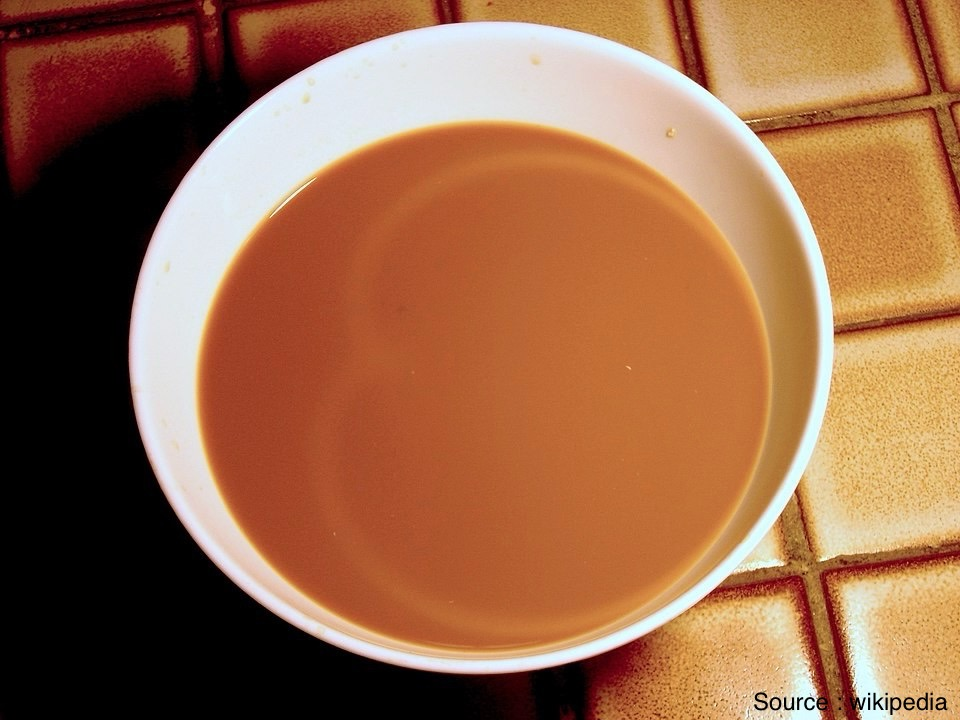
\includegraphics[height=5.0cm]{bol}

\end{frame}

% XXXX
\begin{frame}
\frametitle{\bf XXXX}
 
\centering \includegraphics[height=5.0cm]{xxxx}

\end{frame}

% XXXX
\begin{frame}
\frametitle{\bf XXXX}
 
\centering \includegraphics[height=5.0cm]{xxxx}

\end{frame}

% XXXX
\begin{frame}
\frametitle{\bf XXXX}
 
\centering \includegraphics[height=5.0cm]{xxxx}

\end{frame}

% XXXX
\begin{frame}
\frametitle{\bf XXXX}
 
\centering \includegraphics[height=5.0cm]{xxxx}

\end{frame}

% XXXX
\begin{frame}
\frametitle{\bf XXXX}
 
\centering \includegraphics[height=5.0cm]{xxxx}

\end{frame}

% XXXX
\begin{frame}
\frametitle{\bf XXXX}
 
\centering \includegraphics[height=5.0cm]{xxxx}

\end{frame}

% XXXX
\begin{frame}
\frametitle{\bf XXXX}
 
\centering \includegraphics[height=5.0cm]{xxxx}

\end{frame}

% XXXX
\begin{frame}
\frametitle{\bf XXXX}
 
\centering \includegraphics[height=5.0cm]{xxxx}

\end{frame}

% Once upon a time...
\begin{frame}
\frametitle{\bf Once upon a time...}
 
... there were three little GDRs:
\begin{itemize}
  \item GDR MOA (Math\'ematiques de l'Optimisation et Applications)
  \item GDR CalVa (Calcul des Variations et th\'eorie g\'eom\'etrique de la mesure)
  \item GDR Jeux (Jeux : Mod\'elisation Math\'ematique et Applications) 
\end{itemize}
 
\centering 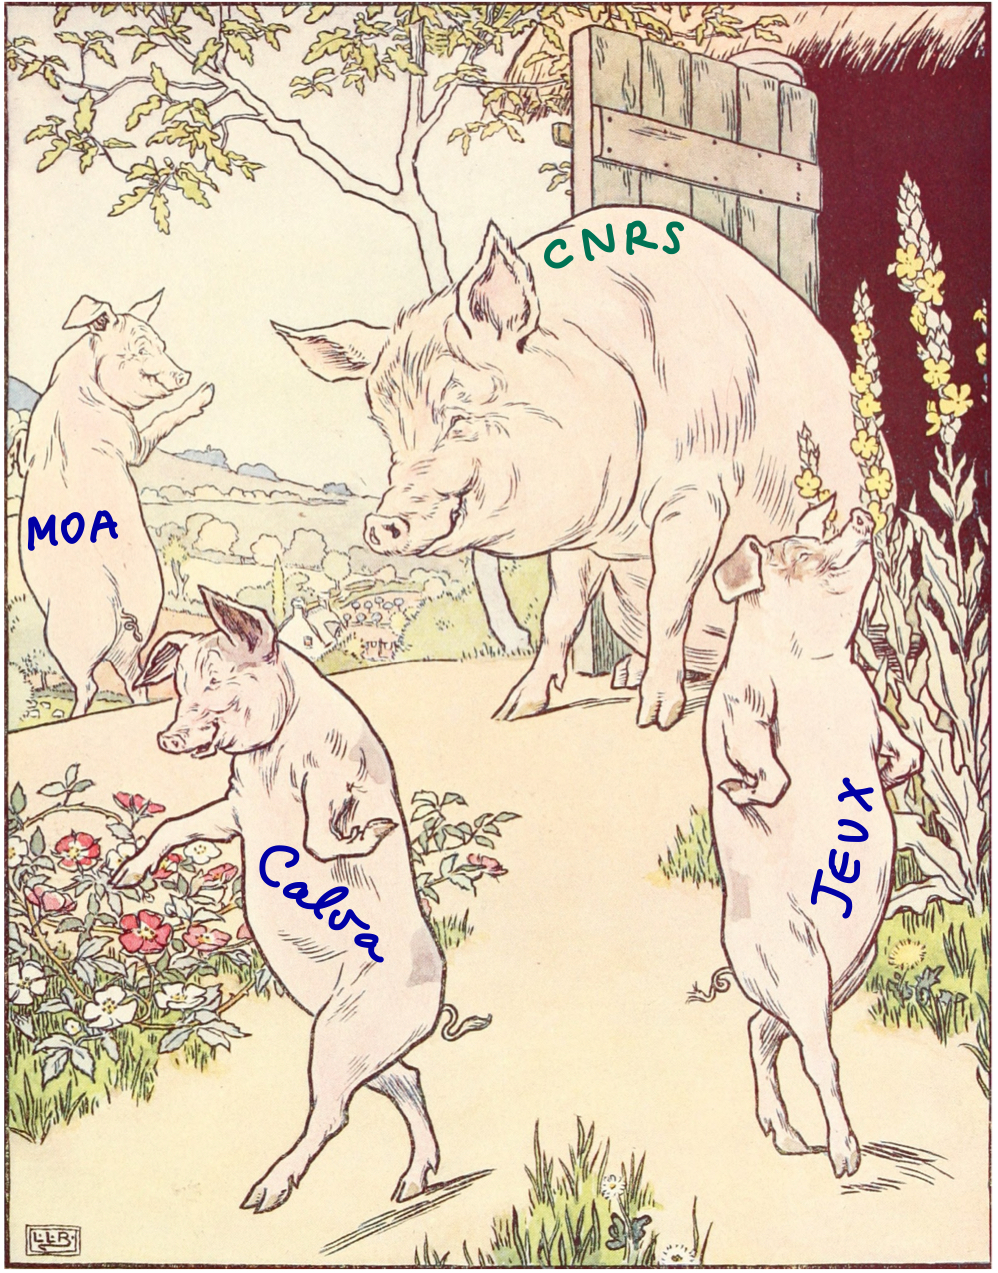
\includegraphics[height=5.0cm]{3-pigs}

\end{frame}

\end{document}

%% - math applis / fonda : obsolète, plutôt pas pertinent
%% - commencer par bol (de la brève : tout autour de la Terre) -> terre plate
%% - explication catacaustique avec dessin
%% - transport optimal : de la géométrie à la pelle (et réciproquement)
%% - monge (cf. liste 4 pb dans ref e ghys) 
%% - existence, unicité, régularité
%% - discret -> continu, plat -> surface avec courbure, [relaxation Kanto / mesure]
%% - villani et al (continuité transport)
%% - cas ellipsoïde pour MTW
%% - applis. : image (continuité !), ML... (G. Peyré, J. Delon pour restauration images...)
%%  Condorcet, « À partir d’applications très simples en apparence, il fait naître l’idée de théories abstraites dont on n’avoit pas encore le besoin [et dirige] vers les théories [les] travaux des Géomètres, et leur [ouvre] une carrière nouvelle ».
%% Poincaré : « Il n’y a pas des problèmes qu’on se pose, il y a des problèmes qui se posent. Il n’y a pas de problèmes résolus, il y a seulement des problèmes plus ou moins résolus ».
%% - carré vers carré (disjoint et orienté différemment) : ouvert
%% - citer refs (Source : XXXX sur image)
%% - transport : cas plat -> surface (variété) : courbure, géodésiques
%% - image : déblai, remblai, pelle
%% - modélisation (cas euclidien)
%% - parcours LMD + MC / CR + HDR + PR / DR
%% - caustique : kaio (je brule)
%% - "le beau, le vrai, l'utile" (Dupin, eleve Monge)
%% - bio
%% Monge est né en 1746 et mort en 1818. 
%% A 18 ans, Monge s’était fait remarquer en dessinant un plan de sa ville natale de Beaune. N’a-t-on pas oublié de nos jours que la géométrie et le dessin ont des liens intimes ? On lui propose alors de venir travailler à l’École du génie de Mézières, non pas comme élève, mais plutôt comme dessinateur ou assistant préparateur.
%% 
%% Voici quelques-uns des mathématiciens de son époque :
%% 
%% Euler : 1707-1783
%% Gauss : 1777-1855
%% 
%% 
%% Jusque 1789, c’est la période qui nous intéressera le plus, celle de la Science. D’abord essentiellement mathématicien, il commencera par la suite, vers 1781, à s’intéresser à la chimie, à la physique, etc. Voici par exemple les titres des mémoires qu’il présente à l’Académie des sciences en 1781 : « machines diverses » ; « sur le froid de 1776 » ; « calcul des chances » ; « machine à remonter les bateaux » ; « moulins à sucre » ; « théorie des torrents et des rivières et moyen d’empêcher leurs ravages ».
%% 
%% La Révolution, sera une période d’engagement politique total. Ce sera l’époque de l’enseignement révolutionnaire, de la fondation de l’École Polytechnique et de l’École Normale de l’an III.
%% 
%% Puis, ce sera la rencontre avec Napoléon Bonaparte, deux longues visites en Italie, la campagne d’Egypte et les honneurs.
%% 
%% Enfin, la Restauration entraînera sa disgrâce. Il meurt en 1818.
%%
%% - refs
%% 
%% https://images-des-maths.pages.math.cnrs.fr/freeze/La-brouette-de-Monge-ou-le-transport-optimal.html
%% 
%% https://images-des-maths.pages.math.cnrs.fr/freeze/Gaspard-Monge,1094.html
%% 
%% https://images-des-maths.pages.math.cnrs.fr/freeze/Gaspard-Monge.html
%% 
%% https://www.gpeyre.com](https://www.gpeyre.com